The distribution of cluster-average Sharpe Ratios across different clusters reveals distinct patterns between KMeans and LLM-based clustering approaches, as illustrated in Figure \ref{fig:cluster-average-SR-by-split}

Panel A presents the results for KMeans clustering, where we observe remarkably consistent distributional patterns across all three data splits. The distributions are approximately symmetric around zero, with the majority of Sharpe ratios falling within the $[-5, 5]$ range. The training set exhibits the highest density peak (approximately $0.17$), followed closely by the test set, while the validation set shows a slightly lower peak density of about $0.125$. Notable in the validation set are small secondary peaks at the tails (around $\pm 15$), suggesting the presence of a few clusters with extreme performance characteristics. This consistency across splits suggests that the KMeans clustering approach produces stable performance groupings.

Panel B displays the results for LLM-based clustering, revealing more heterogeneous distributions across the splits. The validation set demonstrates a pronounced peak near zero with a maximum density of $0.2$, indicating strong concentration of performance in this region. In contrast, the training set exhibits a markedly different pattern, with a flatter, more dispersed distribution extending from $-20$ to $+20$, suggesting greater performance variability across clusters. The test set presents an intermediate case, with moderate concentration around zero but maintaining significant mass in the positive region. This heterogeneity across splits might indicate that the LLM-based clustering captures more nuanced and potentially time-varying patterns in the underlying data.

The contrasting patterns between the two clustering approaches suggest different strengths: KMeans provides more stable and consistent performance groupings, while LLM-based clustering potentially captures more complex relationships, albeit with greater variability across different data splits.
%----------------------------------------------------
\inserthere{fig:cluster-average-SR-by-split}

\begin{figure}[htbp]
\caption{Distribution of Cluster-Average Sharpe Ratios $(\overline{SR}_g)$ by Split}
\label{fig:cluster-average-SR-by-split}

\begin{subfigure}[t]{0.49\textwidth}
\caption{Panel A: KMeans Clustering}
\centering
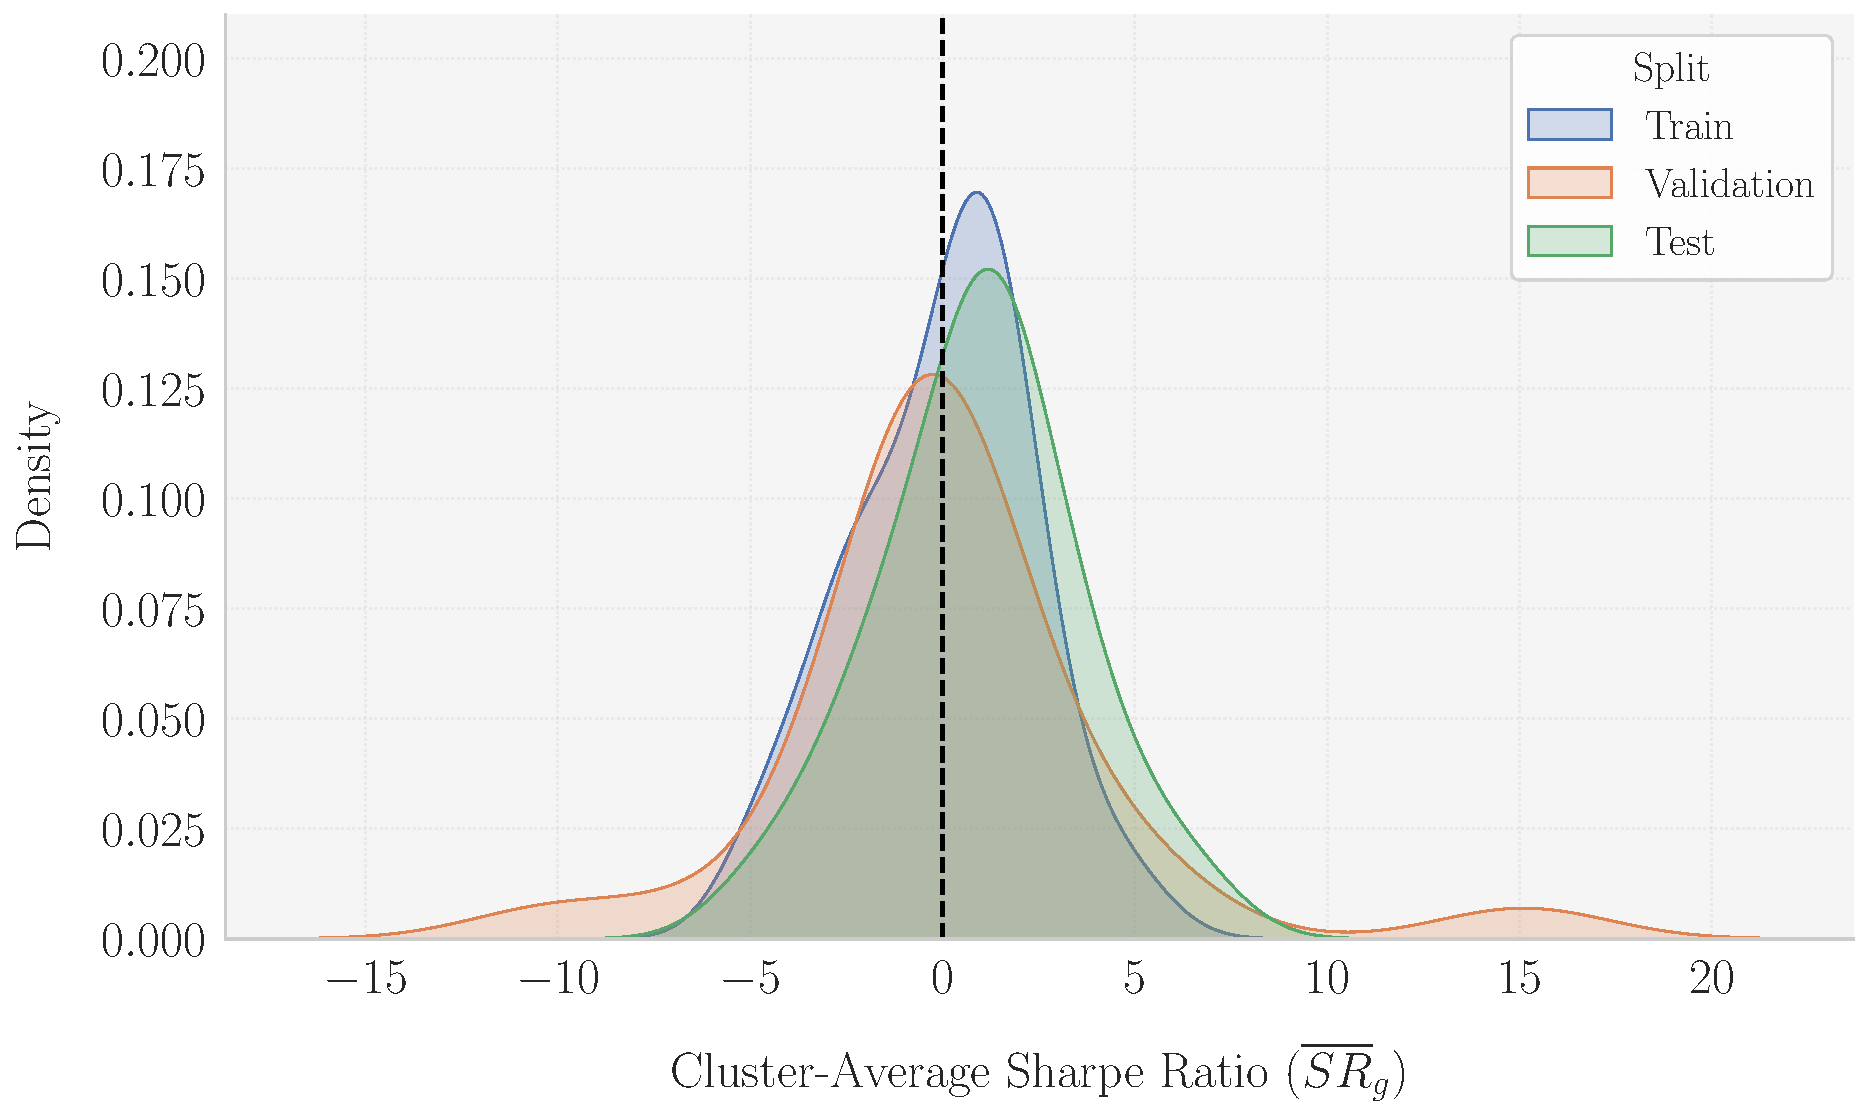
\includegraphics[width=\textwidth]{fig_A5a_KMeans_Cluster-Avg_SR_Distribution.pdf}
\end{subfigure}
\hfill
\begin{subfigure}[t]{0.49\textwidth}
\caption{Panel B: LLM Clustering}
\centering
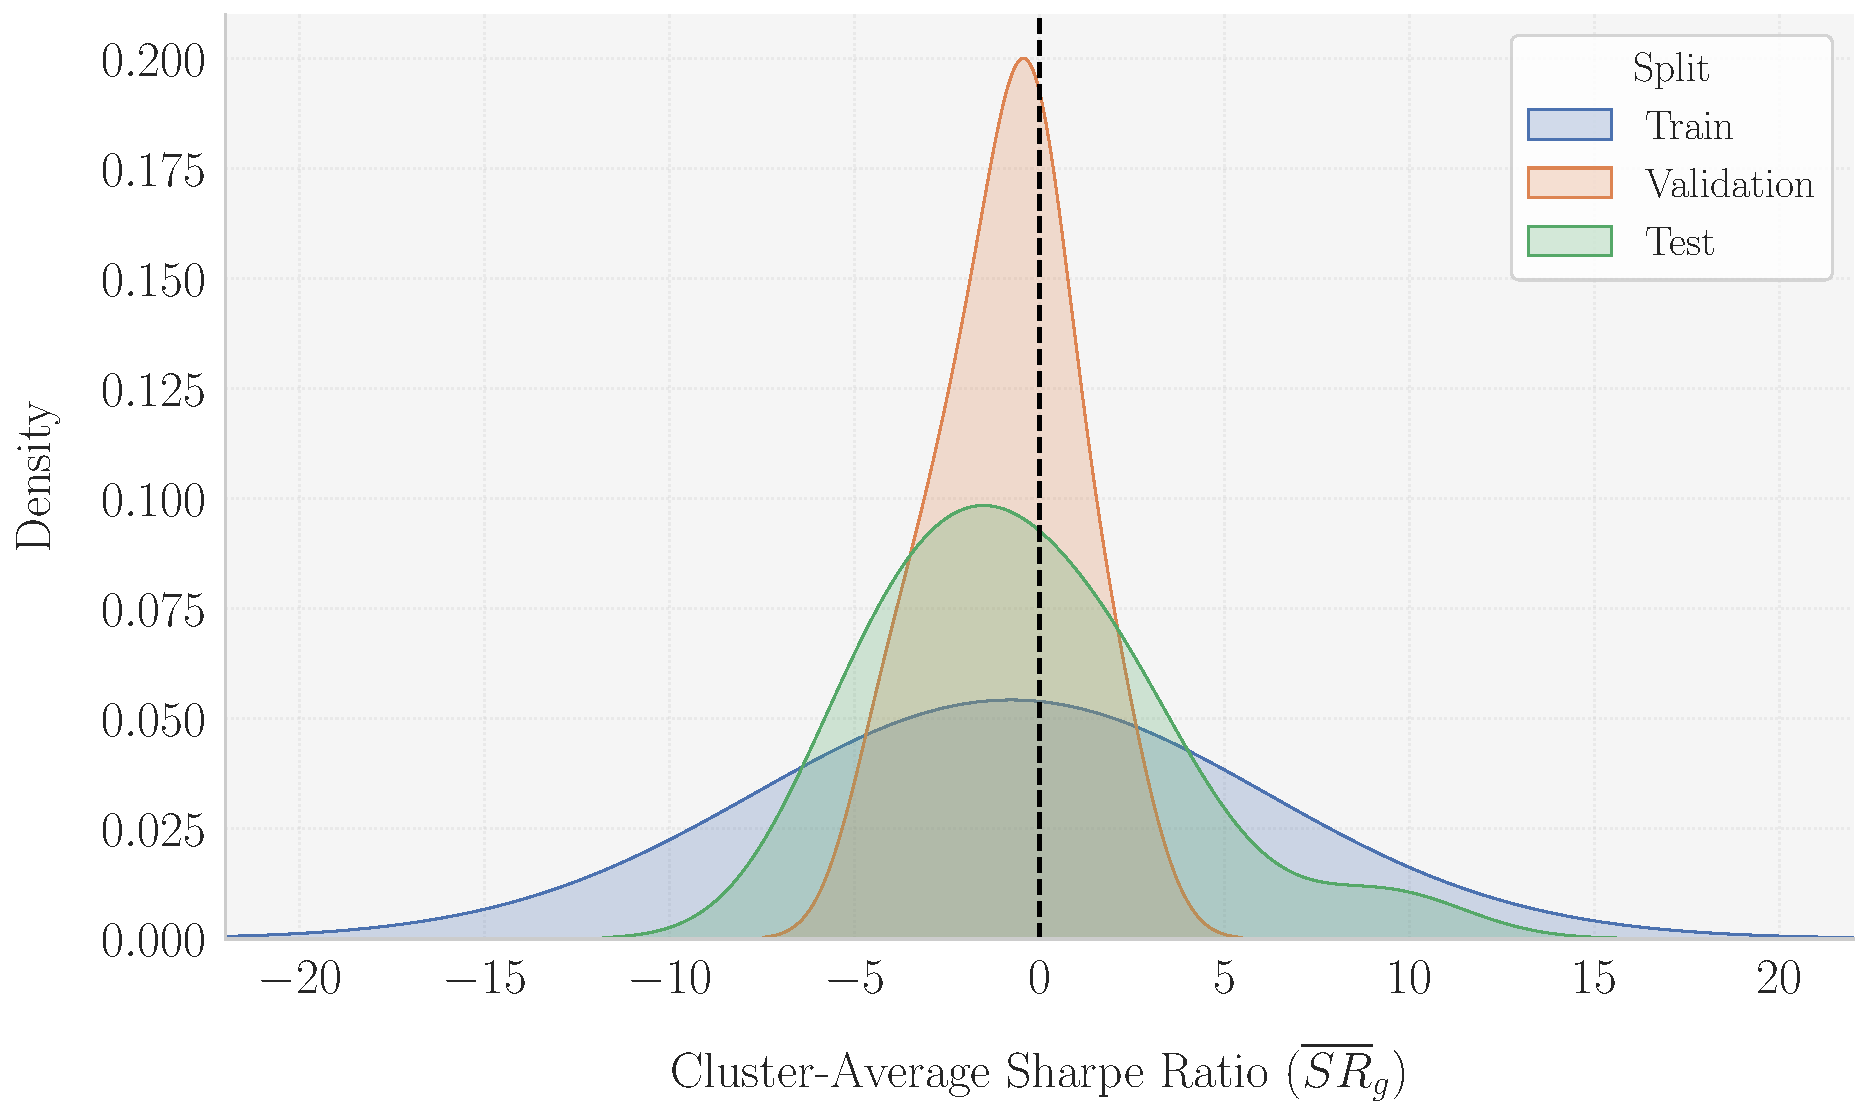
\includegraphics[width=\textwidth]{fig_A5b_LLAMA_Cluster-Avg_SR_Distribution.pdf}
\end{subfigure}

\vspace{0.5cm}
\begin{minipage}{\textwidth}
\setlength{\parindent}{0pt}
{\footnotesize\textit{Note:
This figure presents the distribution of cluster-average Sharpe Ratios $(\overline{SR}_g)$ across training, validation, and test data splits for both KMeans clustering (Panel A) and LLM clustering (Panel B). Each Sharpe Ratio is computed as the average of beta-neutral positions associated with articles in a given cluster. The KMeans approach (Panel A) shows distributions centered around 0 in the validation set, with some outliers exhibiting unusually high or low Sharpe Ratios. The training and test set distributions are slightly right-skewed, suggesting better performance in certain clusters, with no significant outliers. In contrast, the LLM clustering (Panel B) exhibits left-skewed distributions across all splits, indicating a higher frequency of lower Sharpe Ratios. The training data shows fat tails, suggesting extreme values, while the validation data has lighter tails. The test data distribution is more bell-shaped, with Sharpe Ratios concentrated between 5 and 15, indicating stronger performance in some clusters.
}}
\end{minipage}
\end{figure}
%----------------------------------------------------